\section{研究背景及意义}

\subsection{视觉跟踪}

\begin{frame}{视觉跟踪的研究内容}

\begin{block}{}
    视觉跟踪即连续不断地定位运动目标。给定第一帧中的目标位置,跟踪算法能够在视频中预测出目标运动。
\end{block}
\begin{figure}[htp]
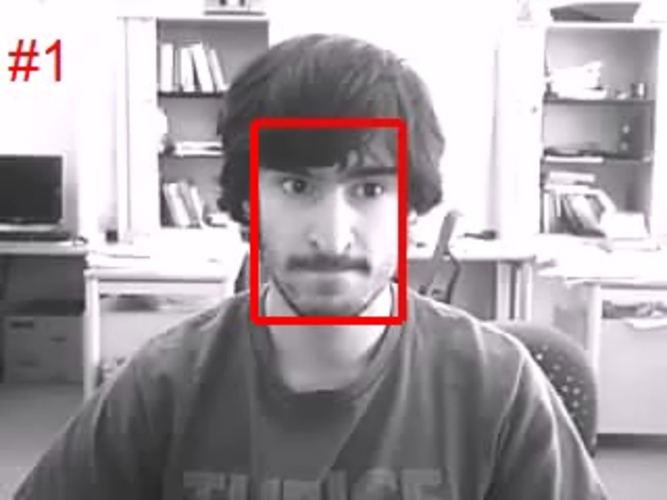
\includegraphics[width=0.25\linewidth,height=0.2\linewidth]{FaceOcc2.pdf}
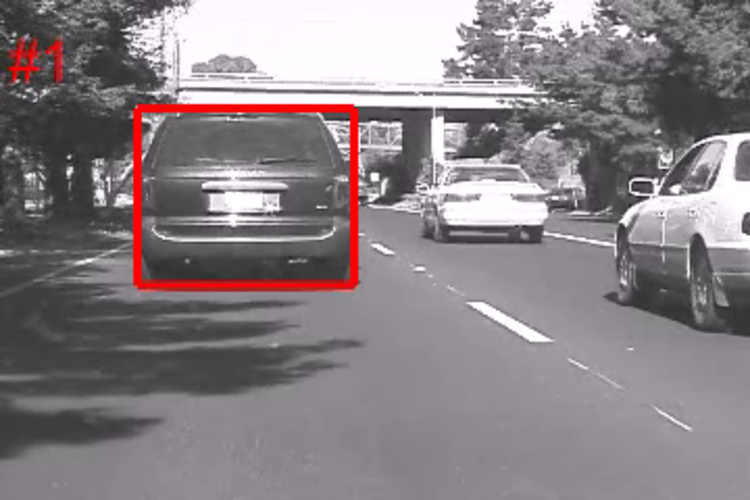
\includegraphics[width =0.25\linewidth,height=0.2\linewidth]{Car4.pdf}
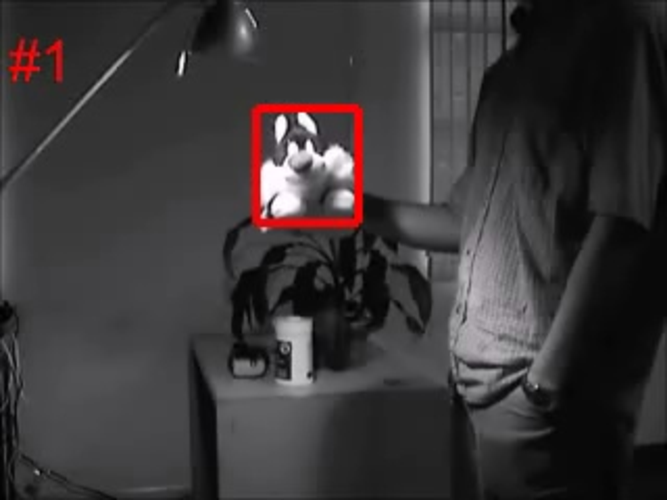
\includegraphics[width =0.25\linewidth,height=0.2\linewidth]{Sylvester.pdf}
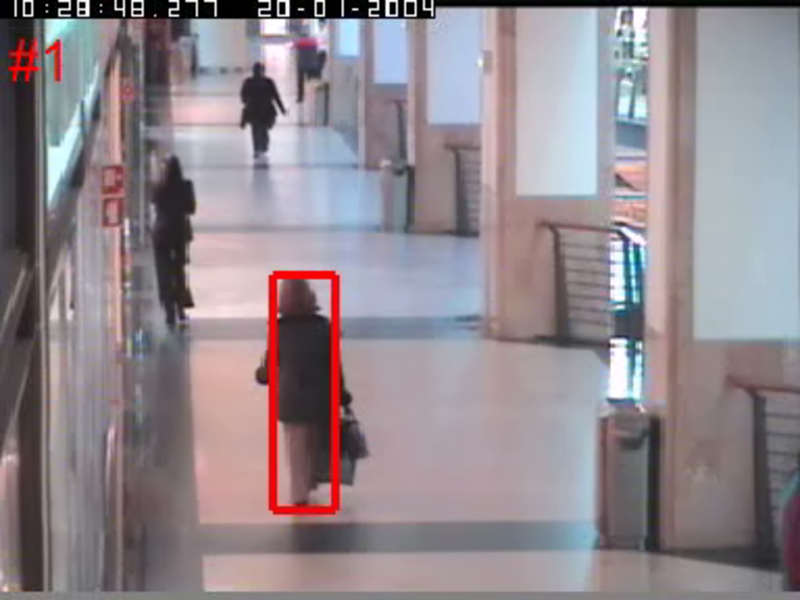
\includegraphics[width =0.25\linewidth,height=0.2\linewidth]{Walking2.pdf}
\caption{单目标视觉跟踪(无模型)}
\end{figure}
\end{frame}


\begin{frame}{视觉跟踪的应用}
    \begin{block}{}
跟踪是视觉监控系统的主要组成部分;在自动驾驶系统中,实时跟踪车辆并预测其运动是非常重要的;自主机器人跟踪它们周围的对象,以便识别人的意图;医学数据分析需要使用可变形模板来跟踪非刚性结构。
\end{block}
\begin{figure}[htp]
%\begin{minipage}{1.06\textwidth}
\subfloat[自动驾驶]{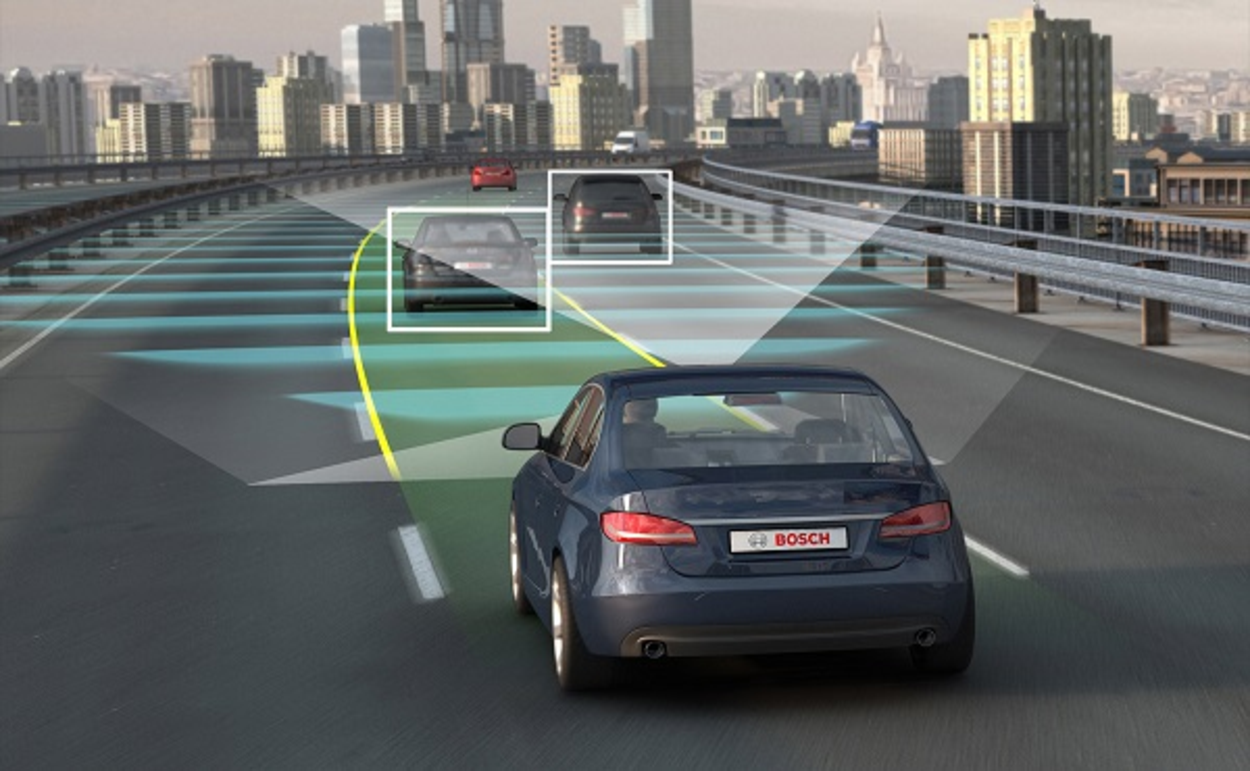
\includegraphics[width=0.25\linewidth,height=0.2\linewidth]{AutonomousCar.pdf}}
\subfloat[人机交互]{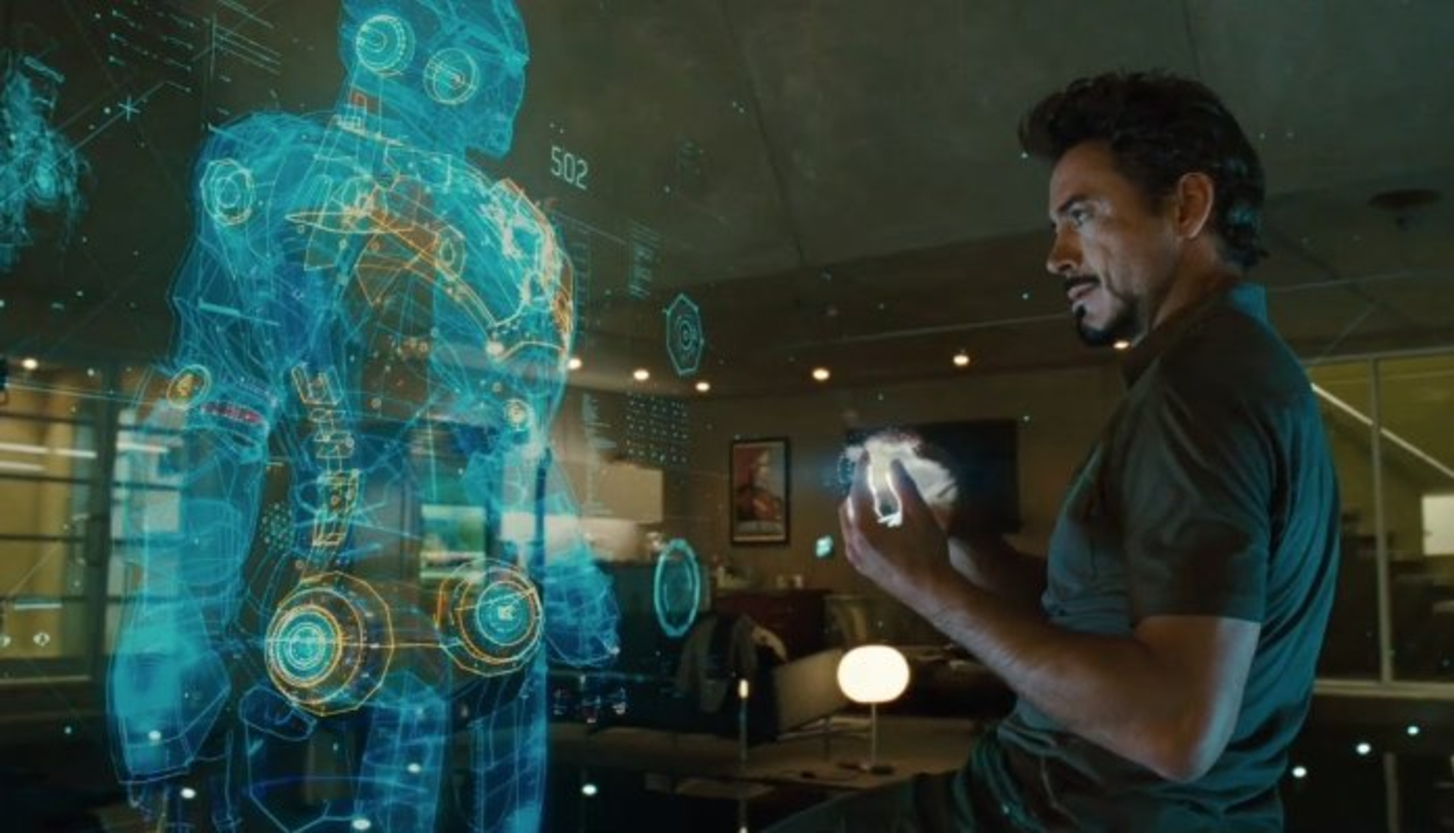
\includegraphics[width =0.25\linewidth,height=0.2\linewidth]{HumanComputerInteraction.pdf}}
\subfloat[运动分析]{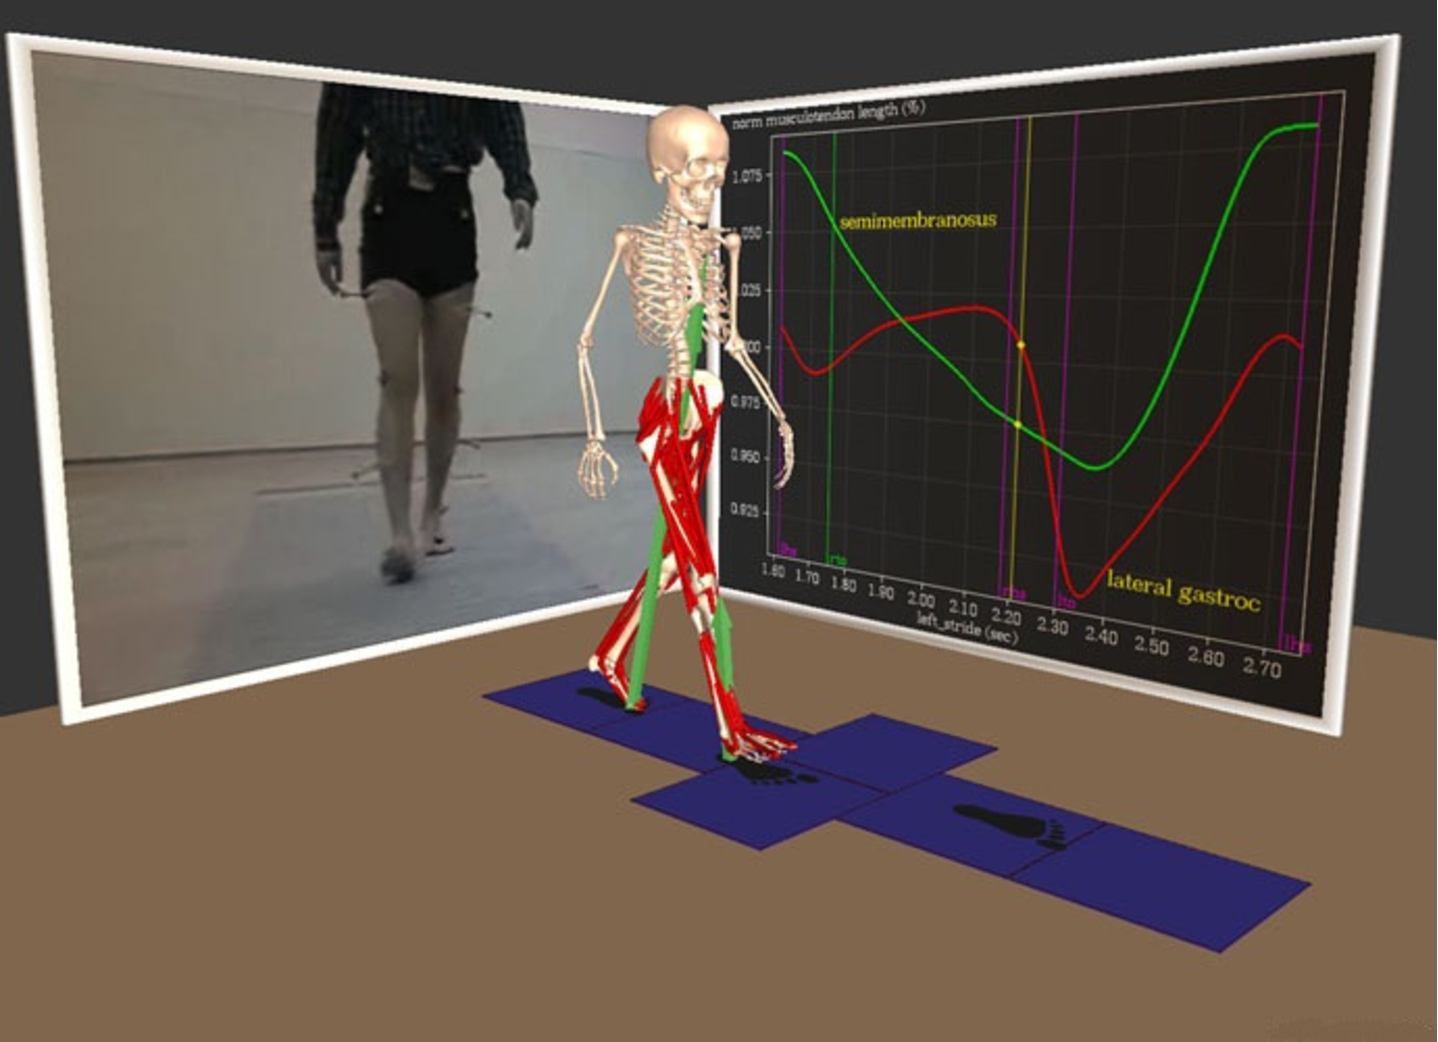
\includegraphics[width =0.25\linewidth,height=0.2\linewidth]{MotionModule.pdf}}
\subfloat[智能监控]{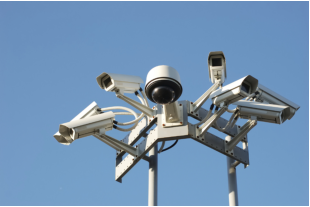
\includegraphics[width =0.25\linewidth,height=0.2\linewidth]{Surveillance.pdf}}
\caption{视觉跟踪的实际应用}
\label{fig:gen_applications}
\end{figure}
\end{frame}

%\begin{frame}{视觉跟踪中的挑战}

%一个良好的跟踪系统需要满足以下要求:

%\begin{block}{鲁棒性}

%鲁棒性意味着即使在复杂的条件下,跟踪算法也能够跟踪感兴趣的对象。跟踪困难可能是杂乱的背景、局部或整体光照变化、遮挡以及复杂的物体运动。
%\end{block}

%\begin{block}{适应性}

%除了对象所处环境的各种变化之外,对象本身也经历变化。这就需要跟踪系统对物体外观拥有稳定的适应机制。
%\end{block}

%\begin{block}{实时性}

%实时处理实时视频流的系统必须具有高处理速度。因此,除了高性能的算法,还需要快速和优化的实现。为了实现对于人眼而言的平滑的视频输出,必须建立至少每秒15帧的帧率。
%\end{block}

%\end{frame}
 
%\subsection{国内外研究现状}

%\begin{frame}{跟踪算法模型}

%\begin{block}{}
%自20世纪80年代以来,已有很多视觉跟踪算法提出。根据模型构建机制的不同,跟踪算法可以分为两类:生成式方法和判别式方法。生成式跟踪器通过搜索最佳匹配窗口执行跟踪,判别式方法依靠学习从背景中区分出目标。
%\end{block}

%\centering
%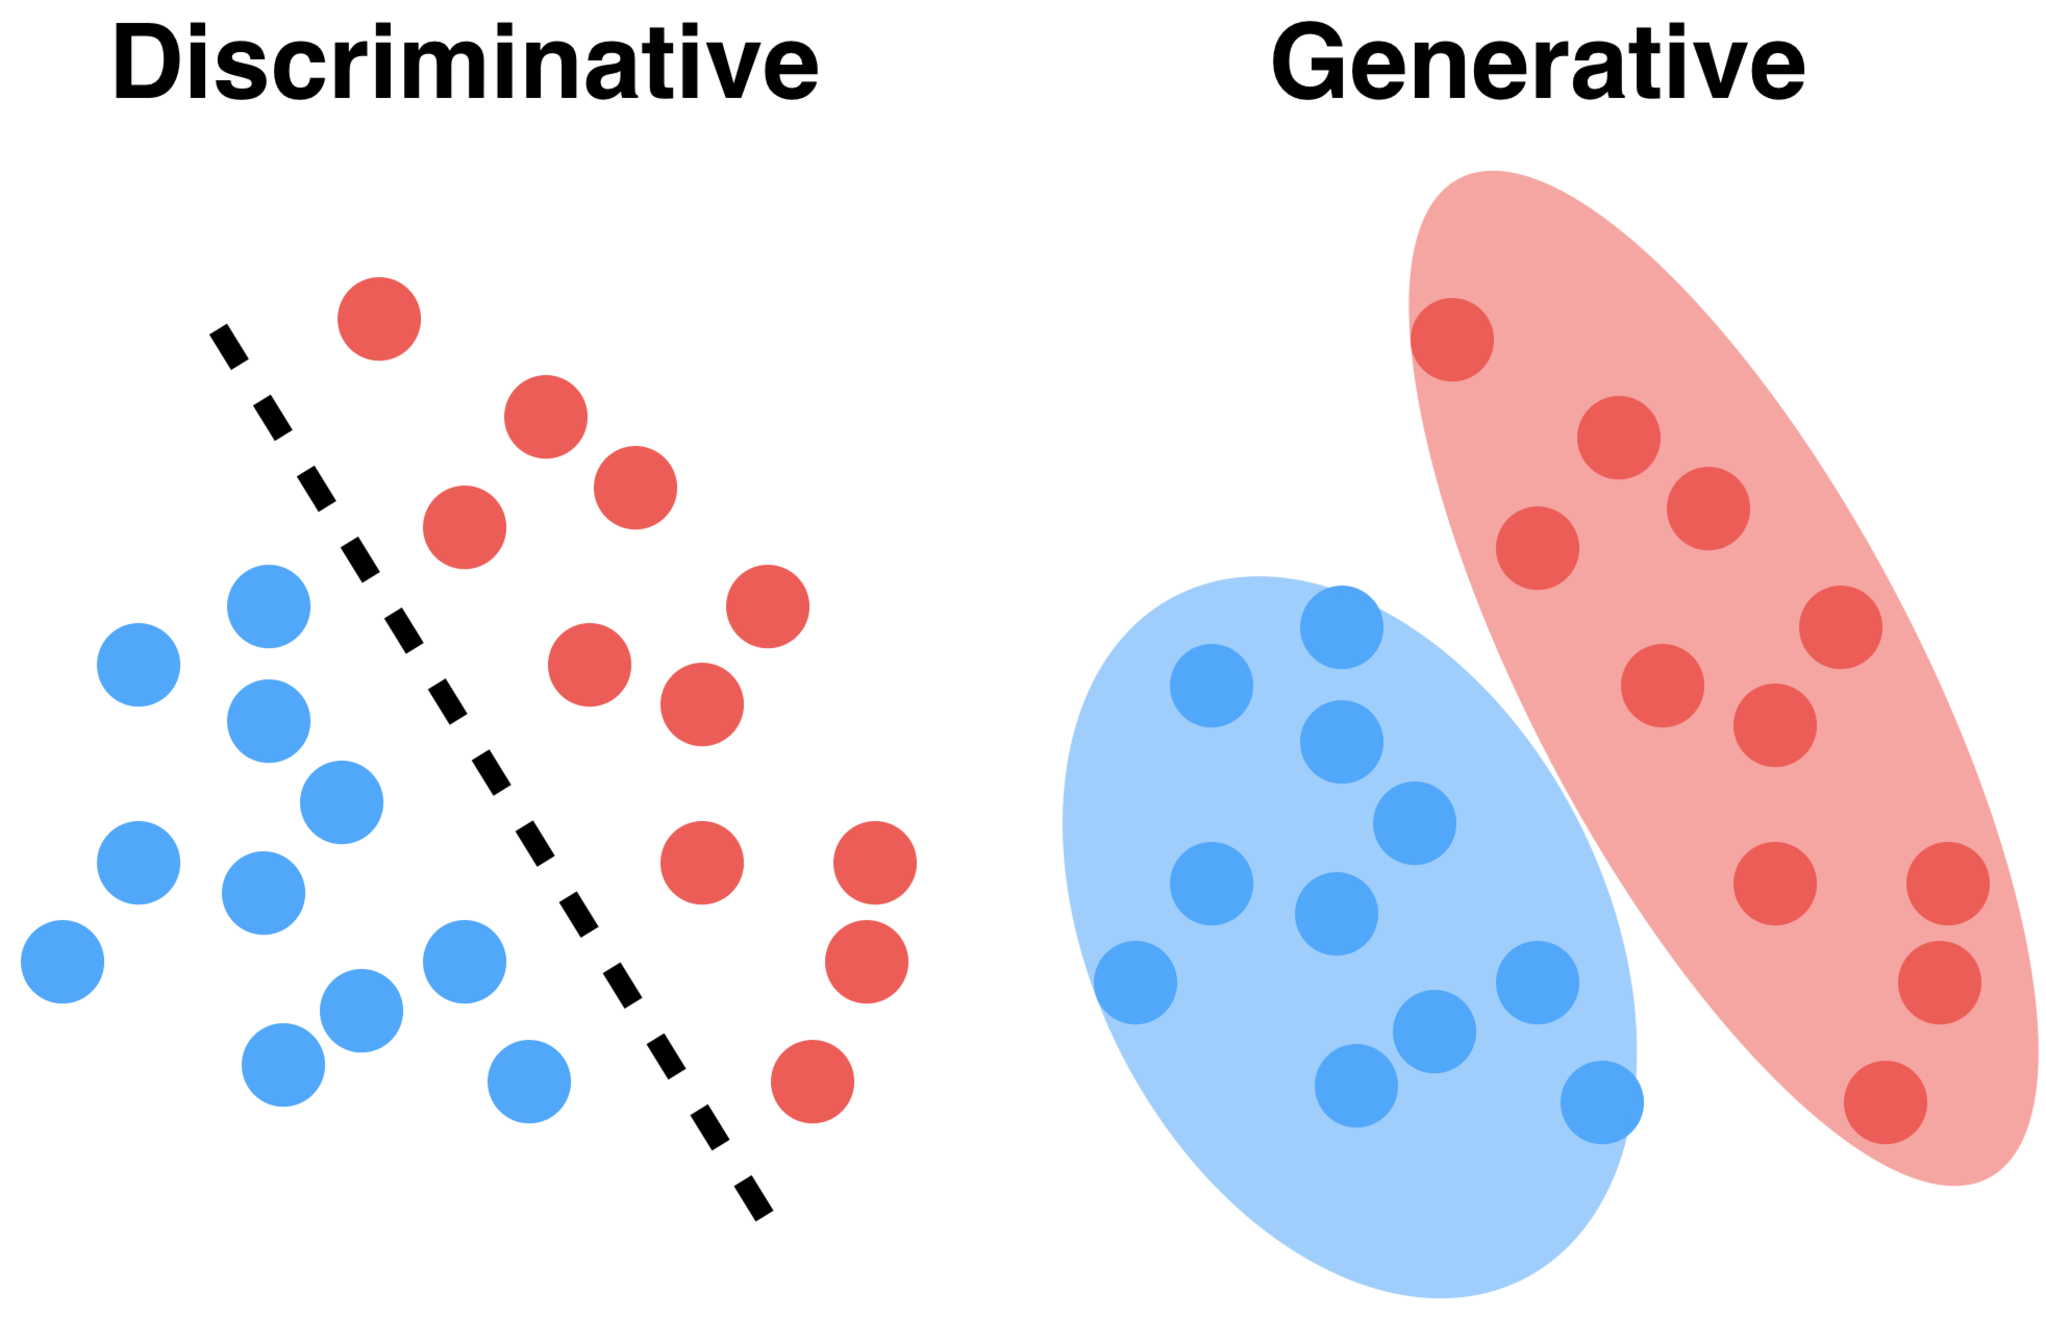
\includegraphics[width =0.5\textwidth,height =0.32\textwidth]{Discriminative_generative.pdf}

%\end{frame}

